
\documentclass[tikz,border=3mm]{standalone}
\begin{document}
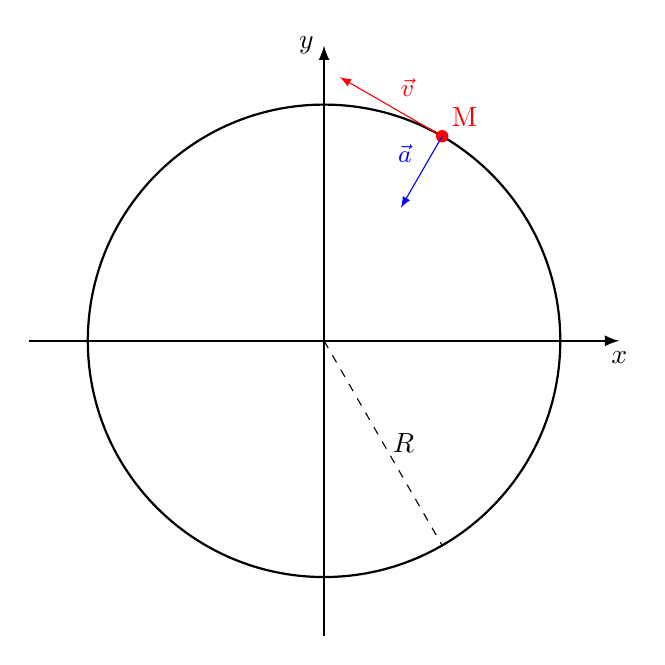
\begin{tikzpicture}[scale=1.5,>=latex]
    % Axes
    \draw[->,thick] (-2.5,0) -- (2.5,0) node[below] {$x$};
    \draw[->,thick] (0,-2.5) -- (0,2.5) node[left] {$y$};

    % Cercle trajectoire
    \draw[thick] (0,0) circle (2cm);

    % Point matériel
    \coordinate (M) at (60:2);
    \coordinate (N) at (-60:2);

    \fill[red] (M) circle (1.5pt) node[above right] {M};

    % Vecteurs
    \draw[->,red] (M) -- ++(150:1) node[midway, above right] {\small $\vec{v}$};
    \draw[->,blue] (M) -- ++(240:0.7) node[midway,above left] {\small $\vec{a}$};

    % Rayon
    \draw[dashed] (0,0) -- (N) node[midway,right] {$R$};



\end{tikzpicture}
\end{document}
